\documentclass[a4paper, 12pt]{article}

\usepackage{titling}
\usepackage{geometry}
\usepackage{graphicx}
\pagenumbering{gobble}

\newcommand{\subtitle}[1]{% 
	\posttitle{%
		\par \end{center}
		\begin{center}\small#1\end{center}
		\vskip7em}%
}


\begin{document}
% Page 1 begins

\title{\Large Digital Signal Processing Project on}
\subtitle{\Huge Huffman Encoding \& Decoding using MATLAB}
\author{\LARGE By:  Ravi Teja Gannavarapu}
\date{\Large Student ID: B216023}
\maketitle

\begin{center}
\Large Branch: Electronics \& Telecommunication Engineering
\newline
Class: 2016 - 2020
\end{center}

\pagebreak
% Page 2 - Abstract

\newgeometry{left=1cm, right=1cm, top=2cm, bottom=2cm}
\pagenumbering{arabic}
\begin{center}
\LARGE Huffman Encoding \& Decoding using MATLAB\\\rule{19cm}{0.01cm}
\end{center}
\begin{center}
\Large Abstract\\\rule{19cm}{0.01cm}\\\vskip2em
\end{center}

\Large Data, when being transmitted over large distances and via different channels, requires to be sent securely. Encoding the
information before transmission is necessary to ensure data security and efficient delivery of the information. \textbf{Huffman algorithm} is a popular encoding method used in communication systems. Huffman encoding and decoding algorithm is used in compressing data with variable-length codes. The shortest codes are assigned to the most frequent characters and the longest codes are assigned to infrequent characters. Huffman coding is an entropy encoding algorithm used for \textbf{lossless} data compression. \textbf{Entropy} is a measure of the unpredictability of an information stream. Maximum entropy occurs when a stream of data has totally unpredictable bits. A perfectly consistent stream of bits (all zeroes or all ones) is totally predictable, and has no entropy.

\pagebreak
% Page 3 - Introduction

\begin{center}
\LARGE Huffman Encoding \& Decoding using MATLAB\\\rule{19cm}{0.01cm}
\end{center}
\begin{center}
\Large Introduction\\\rule{19cm}{0.01cm}\\\vskip2em
\end{center}

\Large Encoding the information before transmission is necessary to ensure data security and efficient delivery of the information. The MATLAB program presented further encodes and decodes the information and also outputs the values of \textbf{entropy, efficiency} and \textbf{frequency probabilities} of characters present in the data stream.
\newline
\newline

Huffman algorithm is a popular encoding method used in communication systems. It is widely used in all the mainstream compression formats that you might encounter - from GZIP, PKZIP and BZIP2, to image formats such as JPEG and PNG. Some programs use just the Huffman coding method, while others use it as one step in a multistep compression process.
\newline
\newline

Huffman encoding \& decoding algorithm is used in compressing data with variable-length codes. The shortest codes are assigned to the most frequent characters and the longest codes are assigned to infrequent characters.
\newline
\newline

Huffman coding is an entropy encoding algorithm used for lossless data compression. \textbf{Entropy} is a measure of the unpredictability of an information stream. Maximum entropy occurs when a stream of data has totally unpredictable bits. A perfectly consistent stream of bits (all zeroes or all ones) is totally predictable (has no entropy).

\pagebreak
% Page 4 - Huffman Tree

\begin{center}
\LARGE Huffman Encoding \& Decoding using MATLAB\\\rule{19cm}{0.01cm}
\end{center}
\begin{center}
\Large Huffman Tree\\\rule{19cm}{0.01cm}\\\vskip2em
\end{center}

\Large The Huffman coding method is somewhat similar to the Shannon–Fano method. The main difference between the two methods is that Shannon–Fano constructs its codes from top to bottom (and the bits of each codeword are constructed from left to right), while Huffman constructs a code tree from the bottom up and the bits of each codeword are constructed from right to left.
\newline
\newline

The simplest tree construction algorithm uses a priority queue or table where the node with the lowest probability or frequency is given the highest priority. First, create a leaf node for each symbol or character and add it to the priority table. If there is more than one node in the table, remove two nodes of the highest priority (lowest frequency) from the table. Create a new node with these two nodes as sub-nodes and with probability equal to the sum of the two nodes’ probabilities. Continue in this way until you reach the last single node. The last node is the root, so the tree is now complete.
\newline
\newline

\begin{center}
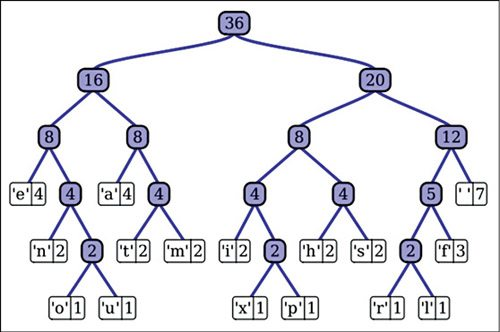
\includegraphics[width=300px]{huffmantree.jpg}
\end{center}
\begin{center}
\large Figure 1: Huffman Tree.
\end{center}

\pagebreak
% Page 5 - Steps to encode

\begin{center}
\LARGE Huffman Encoding \& Decoding using MATLAB\\\rule{19cm}{0.01cm}
\end{center}
\begin{center}
\Large Steps to encode\\\rule{19cm}{0.01cm}\\\vskip2em
\end{center}

\begin{enumerate}
\item Compute the probability of each character in a set of data.
\item Sort the set of data in ascending order.
\item Create a new node where the left sub-node is the lowest frequency in the sorted list and the right sub-node is the second lowest in the sorted list.
\item Remove these two elements from the sorted list as they are now part of one node and add the probabilities. The result is the probability for the new node.
\item Perform insertion sort on the list.
\item Repeat steps 3, 4 and 5 until you have only one node left.
\end{enumerate}

Now that there is one node remaining, simply draw the tree. With the above tree, place a ‘0’ on each path going to the left and a ‘1’ on each path going to the right. Now assign the binary code to each of the symbols or characters by counting 0’s and 1’s starting from the root
\newline
\newline

From the above, it is now clear that the encoding method should give rise to a uniquely decodable code so that the original message can be detected uniquely and perfectly without errors. The message generated with the highest probability will be generated more number of times than other messages. In such a case, if you use a variable-length code instead of a fixed-length code, you will be improving the efficiency by assigning fewer bits to the higher-probability messages than the lower-probability messages.

\end{document}